\chapter{Results}
\vspace{10mm}

\begin{quote}
  {\it ``There's a basic rule which runs through all kinds of music, 
    kind of an unwritten rule. I don't know what it is.  But I've got
    it.''} --- Ron Wood, guitarist for the Rolling Stones.
\end{quote}


\vspace{7mm}

The result of this thesis is a software system that 
realizes the algorithms described in the previous chapter. 
The outputs of the software are twofold. First, there is the rhythmic 
timing data extracted from each stream that is saved as a MIDI file or
re-interpreted  with an audio sample and saved as digital audio.
Second, there is the graphical interpretation of the timing data as the 
lowest-level pulse in each stream.

% [Discuss here the process of mixing 3 signals and then running them
% thru ISA and talk about the results]

The quality of the MIDI rendering and the re-interpreted audio files is
very promising.  In most cases, a high quality extraction of an
instrument virtually guarantees clean results from the onset
analysis. Additionally, variable threshold values and minimum
onset spacing parameters add to the robustness of the onset detection
algorithm. The ISA algorithm works especially well when the number of
voices to be separated is low (i.e. less than five). Note that when the
number of voices is much higher, a hierarchical ISA technique 
should be employed. This means that a mono audio file is first run through a
ISA extraction with a low number of components, and each component is
then run through subsequent ISA extractions to further unmix the
latent sources.

The interpretation of the timing data for each stream is also promising.
While not having many practical compositional uses, its
analytic value is important.  For example, an accelerando or
ritardando in an extracted instrument will be seen as an increase or 
decrease respectively in that instrument's lowest level
pulse. In most popular dance and folk music, if one of the extracted 
instruments is a kick drum or some other salient pulse keeper, the
lowest  level pulse is interpreted as the foot-tapping beat or tactus 
of the entire work.

\begin{figure}[thp]
  \begin{center}
    \resizebox{4.5in}{!}{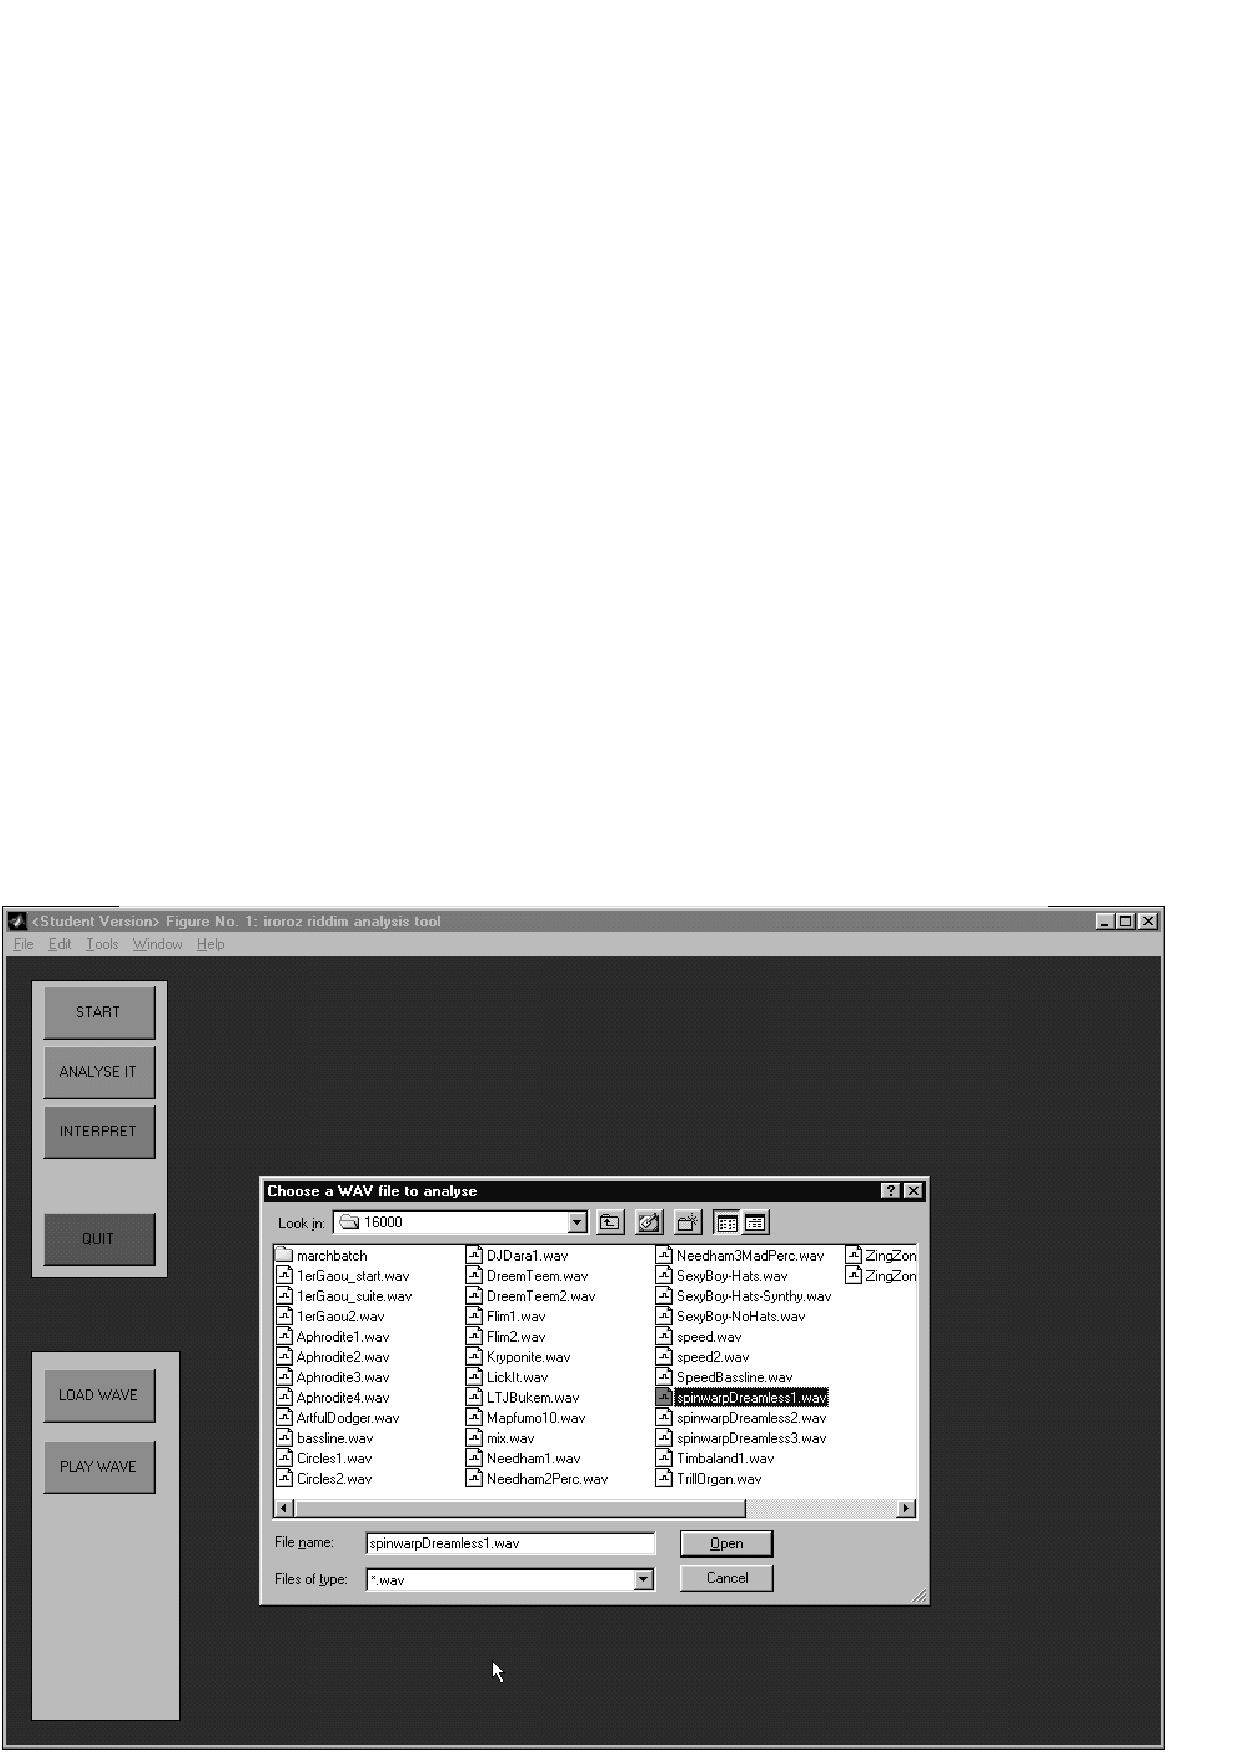
\includegraphics{RiddimScreenStart1.pdf}}
    \caption{A screen shot of {\it Riddim} in the Start Mode, with an
      open dialog box to choose a WAV file to analyse}  
    \label{Riddim Analysis Start Screen Shot}
  \end{center}
\end{figure}




\vspace{7mm}
\section{{\it Riddim}}
\vspace{3mm}

Because {\it Riddim} is also a proof-of-concept for a real-time rhythm
analysis/synthesis engine, the completion of the software goes beyond
the scope of this thesis. For that reason, I will not be including 
the source code in this document. Rather, all the source and examples 
will be distributed on the web under the GNU General Public License
(GPL) agreement, available at \begin{verbatim}
  http://eamusic.dartmouth.edu/~iroro/
\end{verbatim}

{\it Riddim} is organized into three modes, a start, an analysis 
and an interpretation mode. In the start mode, the user can load and
preview audio files.  The user then advances to the analysis mode   
where the loaded audio data is subjected to the algorithms 
discussed in the previous chapters.  The user can enter a set
of variables that direct the course of the analysis algorithms. After
the user pushes ``GO'', the ISA extraction routines proceed and return a
menu allowing the user to select a stream to view. 
By selecting a stream, the onset detection algorithm is run and the 
user is presented with the extracted waveform with superimposed
grid lines indicating onset times. At this stage the
user is can enter a spacing parameter and a threshold value to
fine tune the quality of the onset detection. The user change also
change the parameters used for the ISA extraction by hitting
``GO'' to re-run the analysis. \begin{figure}[thp]
  \begin{center}
    \resizebox{4.5in}{!}{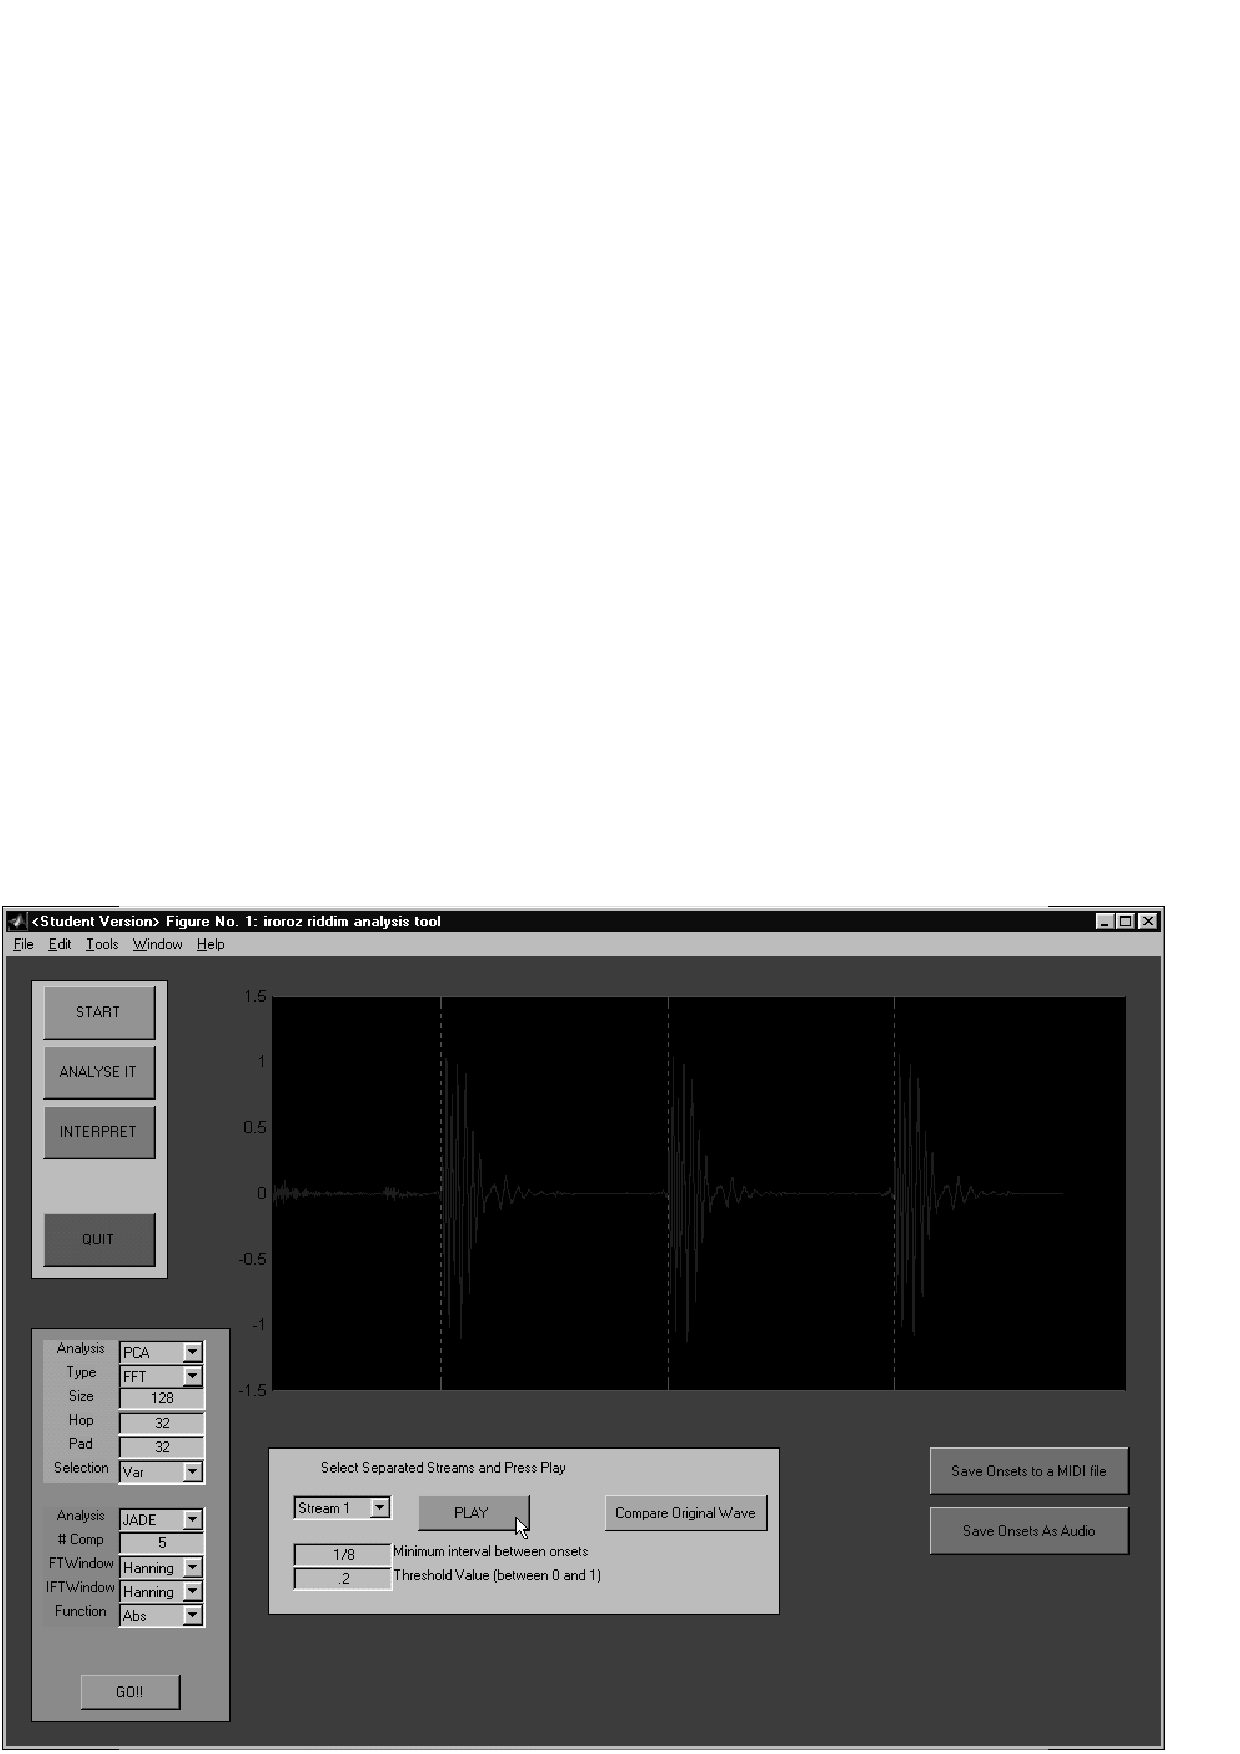
\includegraphics{RiddimScreenAnalyse1.pdf}}
    \caption{A screen shot of {\it Riddim} in the Analysis Mode. Shown
      are an extracted kick drum and the detected onsets indicated by
      the grid lines.} 
    \label{Riddim Analysis Screen Shot}
  \end{center}
\end{figure}
Once the onset times per stream are 
as desired, there are two buttons that allow the timing
information to be saved as a MIDI file or as digital audio.  In the
latter case, a dialog window will appear asking the user to choose a 
file with which to render the timing information. At any stage the
user can load another audio file or reload the current file.

So far these modes embody the functionality of the first high level
subsystem. The next and final mode, the ``Interpretation'' mode, is the
forum for a variety of interpretive analyses of the extracted timing
data. As was discussed above, only the determination of the
lowest-level pulse was implemented. Accordingly, in this mode, the
user is presented with the same menu of extracted streams. This time 
selecting a stream will return the specified stream, the associated 
onsets {\sl and} a plot of the movement of the lowest level
pulse. Refer to Figure \ref{lowestlevelpulse}.


